\PassOptionsToPackage{unicode,pdfusetitle}{hyperref}
\PassOptionsToPackage{hyphens}{url}
\PassOptionsToPackage{dvipsnames,svgnames,x11names}{xcolor}

\documentclass[aspectratio=1610,onlytextwidth]{beamer}

\usetheme{moloch}
\usefonttheme{professionalfonts}
\setbeamertemplate{page number in head/foot}[appendixframenumber]

\usepackage{listings}
\usepackage{lstautogobble}
\lstset{
  autogobble,
  language=R,
  showspaces = false,
  morekeywords={TRUE, FALSE},
  showtabs = false,
  breaklines = true,
  tabsize = 2,
  keywordstyle=\color{SteelBlue4},
  stringstyle=\color{Lavender},
  deletekeywords={data,frame,length,as,character},
  basicstyle=\ttfamily\footnotesize
}

\usepackage{lmodern}
\usepackage{amssymb,amsmath,mathtools,amsthm}
\usepackage[T1]{fontenc}
\usepackage{textcomp}

% \usepackage{minted}

\usepackage{upquote} % straight quotes in verbatim environments
\usepackage{microtype}
\UseMicrotypeSet[protrusion]{basicmath} % disable protrusion for tt fonts

\usepackage{xcolor}
\usepackage{xurl} % add URL line breaks if available
\usepackage{bookmark}
\usepackage{hyperref}

\usepackage{tikz}

\hypersetup{%
  colorlinks = true,
  linkcolor  = mLightGreen,
  filecolor  = mLightGreen,
  citecolor  = mLightGreen,
  urlcolor   = mLightGreen
}

% animations
\usepackage{xmpmulti}

%% subfigures
% \usepackage{subcaption}

% algorithms
\usepackage[ruled,vlined]{algorithm2e}
\resetcounteronoverlays{algocf}

\usepackage{booktabs}

\date{\today}
\titlegraphic{\hfill
\includegraphics[width=4cm]{images/ucph-horizontal-right.pdf}\vspace{1cm}}

% bibliography
\usepackage[style=authoryear]{biblatex}
\addbibresource{lecture13.bib}

% title block
\title{Variations on Stochastic Gradient Descent}
\subtitle{Computational Statistics}
\author{Johan Larsson}
\institute{Department of Mathematical Sciences, University of Copenhagen}

% operators
\DeclareMathOperator*{\argmax}{arg\,max}
\DeclareMathOperator{\diag}{diag}

% macros
\newcommand{\pkg}[1]{\textsf{#1}}
\renewcommand{\vec}{\vectorsym}
\newcommand{\mat}{\matrixsym}
\newcommand{\du}{\mathrm{d}}


\begin{document}

\maketitle

% \begin{frame}[c]
%   \frametitle{Overview}
%
%   \tableofcontents
% \end{frame}
%
\begin{frame}[c]
  \frametitle{Errata}
  \begin{itemize}
    \item There is rationale for step size differences in least squared loss and
          log-likelihood loss: gradients are larger in former.
  \end{itemize}
\end{frame}

\begin{frame}[c]
  \frametitle{Last Time}

  \begin{columns}[T]
    \begin{column}{0.39\textwidth}
      \begin{block}{SGD}
        Introduced stochastic gradient descent (SGD) and mini-batch version thereof.
      \end{block}
      \pause
      \begin{block}{Problems}
        We indicated that there were problems with vanilla SGD: poor convergence,
        erratic behavior.
      \end{block}
    \end{column}
    \begin{column}{0.51\textwidth}
      \begin{algorithm}[H]
        \KwData{$\gamma_0 >0$ }
        \For{$k \gets 1, 2, \dots$}{
          $A_k \gets$ random mini-batch of $m$ samples\;
          $x_k \gets x_{k-1} - \frac{\gamma_k }{|A_k|} \sum_{i \in A_k} \nabla f_i(x_{k-1})$\;
        }
        \caption{Mini-Batch SGD}
      \end{algorithm}
    \end{column}
  \end{columns}

\end{frame}

\begin{frame}[c]
  \frametitle{Today}

  How can we improve stochastic gradient descent?

  \begin{block}{Momentum}
    Base update on combination of gradient step and previous point.

    \medskip

    Two versions: Polyak and Nesterov momentum
  \end{block}

  \pause

  \begin{block}{Adaptive Gradients}
    Adapt learning rate to particular feature.
  \end{block}

\end{frame}

\begin{frame}
  \frametitle{Momentum}

  \begin{columns}
    \begin{column}{0.45\textwidth}
      \begin{block}{Basic Idea}
        Give the particle \textbf{momentum}: like a heavy ball

        \medskip

        Not specific to stochastic GD!
      \end{block}

      \pause

      \begin{block}{Polyak Momentum}
        Classical version

        \medskip

        $\mu \in [0, 1)$ decides strength of momentum; $\mu = 0$ gives standard gradient descent

        \medskip

        Typically let $x_{-1} = x_{0}$.

        \medskip

        Guaranteed convergence for quadratic functions
      \end{block}
    \end{column}
    \begin{column}{0.45\textwidth}
      \begin{algorithm}[H]
        \KwData{$\gamma >0$, $\mu \in [0,1)$}
        \For{$k \gets 1, 2, \dots$}{
          $x_k \gets x_{k-1} - \gamma  \nabla f(x_{k-1}) + \mu (x_{k-2} - x_{k-2}) $\;
        }
        \caption{GD with Polyak Momentum}
      \end{algorithm}
    \end{column}
  \end{columns}

\end{frame}

\begin{frame}[c]
  \frametitle{Polyak Momentum in Practice}

  \begin{figure}[htpb]
    \centering
    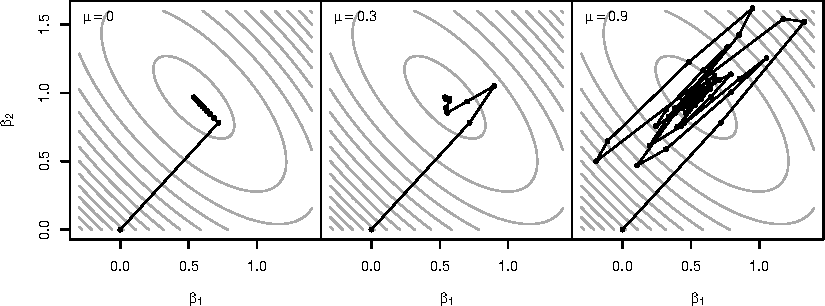
\includegraphics[]{images/momentum-surface.pdf}
    \caption{%
      Trajectories of GD for different momentum values for a least-squares problem
    }
  \end{figure}

\end{frame}

\begin{frame}[c]
  \frametitle{Local Minima}

  \begin{columns}
    \begin{column}{0.45\textwidth}
      For nonconvex \(f\), gradient descent may get stuck at a local minimum.
    \end{column}

    \begin{column}{0.45\textwidth}
      \begin{figure}[htpb]
        \centering
        \multiinclude[<+>][format=pdf]{images/escape-minima-gd}
        \caption{%
          $\mu = 0$
        }
      \end{figure}
    \end{column}
  \end{columns}

\end{frame}

\begin{frame}[c]
  \frametitle{Escaping Local Minima}

  \begin{columns}
    \begin{column}{0.45\textwidth}
      With momentum, we can (sometimes) remedy this problem.
    \end{column}
    \begin{column}{0.45\textwidth}
      \begin{figure}[htpb]
        \centering
        \multiinclude[<+>][format=pdf]{images/escape-minima-mom}
        \caption{%
          $\mu = 0.8$
        }
      \end{figure}
    \end{column}
  \end{columns}

\end{frame}

\begin{frame}[c]
  \frametitle{Convergence Failure}

  \begin{columns}
    \begin{column}{0.45\textwidth}
      For some problems, the momentum method may instead lead to a failure to converge.

      \pause

      \bigskip

      Consider
      \[
        f(x) =
        \begin{cases}
          \frac{25x^2}{2}            & \text{if } x < 1,        \\
          \frac{x^2}{2} +24x - 12    & \text{if } 1 \leq x < 2, \\
          \frac{25x^2}{2} - 24x + 36 & \text{if } x \geq 2.
        \end{cases}
      \]

      \pause
      \bigskip

      For an ``optimal'' step size $1 = 1/ L$ with $L = 25$, GD
      momentum steps converge to three limit points.

    \end{column}
    \begin{column}{0.45\textwidth}
      \begin{figure}[htpb]
        \centering
        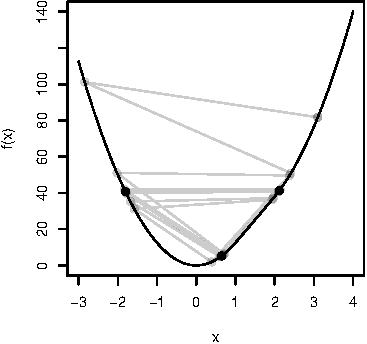
\includegraphics[]{images/momentum-failure.pdf}
        \caption{%
          Initialized at $x_0 = 3.2$, the algorithm fails to converge.
        }
      \end{figure}
    \end{column}
  \end{columns}
\end{frame}

\begin{frame}[c]
  \frametitle{Nesterov Momentum}
  \begin{algorithm}[H]
    \KwData{$\gamma >0$, $\mu \in [0,1)$}
    \For{$i \gets 1,2,\dots$}{
      $v_k \gets x_{k-1} - \gamma \nabla f(x_{k-1})$\;
      $x_k \gets v_{k} + \mu (v_{k} - v_{k-1})$\;
    }
    \caption{GD with Nesterov Momentum}
  \end{algorithm}

  \bigskip

  Overcomes convergence problem of classical (Polyak) momentum.

\end{frame}

\begin{frame}[c]
  \frametitle{Nesterov: Sutskever Perspective}
  \begin{columns}[T]
    \begin{column}{0.45\textwidth}
      Consider two iterations of Nesterov algorithm:
      \[
        \begin{aligned}
          v_{t}               & = x_{t-1} - \gamma \nabla f\left(x_{t-1} \right)         \\
          \alert<2->{x_{t}}   & \alert<2->{= v_{t} + \mu\left(v_{t} - v_{{t-1}} \right)} \\
          \alert<2->{v_{t+1}} & \alert<2->{= x_{t} - \gamma \nabla f\left(x_{t} \right)} \\
          x_{t+1}             & = v_{t+1} + \mu\left(v_{t+1} - v_{t} \right)
        \end{aligned}
      \]
    \end{column}

    \pause

    \begin{column}{0.45\textwidth}
      Idea: focus on interim step:
      \[
        \begin{aligned}
          x_{t}   & = v_{t} + \mu\left(v_{t} - v_{{t-1}} \right) \\
          v_{t+1} & = x_{t} - \gamma \nabla f\left(x_{t} \right)
        \end{aligned}
      \]

      \pause

      Reindex:
      \[
        \begin{aligned}
          x_{t} & = v_{t-1} + \mu\left(v_{t-1} - v_{{t-2}} \right) \\
          v_{t} & = x_{t} - \gamma \nabla f\left(x_{t} \right)
        \end{aligned}
      \]
    \end{column}

  \end{columns}

  \pause \bigskip

  But since $x_k = v_k$ for $k=1$ by construction, we can swap $x_k$ for $v_k$ and
  get the update
  \[
    x_k = x_{k-1} + \mu(x_{k-1} - x_{k-2}) - \gamma \nabla f(x_{k} + \mu(x_{k-1} - x_{k-2})).
  \]
\end{frame}

\begin{frame}[c]
  \begin{figure}[htpb]
    \centering
    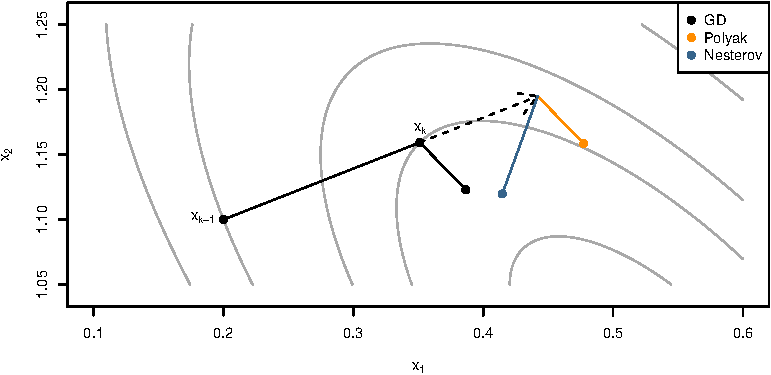
\includegraphics[]{images/momentum-illustration.pdf}
    \caption{%
      Illustration of Nesterov and Polyak momentum
    }
  \end{figure}
\end{frame}

\begin{frame}[c]
  \frametitle{Optimal Momentum}
  \begin{columns}
    \begin{column}{0.45\textwidth}
      For gradient descent with \(\gamma = 1/L\), the optimal choice of \(\mu_k\) for
      general convex and smooth \(f\) is
      \[
        \mu_k = \frac{a_{k-1} - 1}{a_{k}}
      \]
      for a series of
      \[
        a_k = \frac{1 + \sqrt{4a_{k-1}^2 + 1}}{2}
      \]
      with \(a_1 = 1\) (and hence \(\mu_1 = 0\)).

      \bigskip\pause

      First step (\(k = 1\)) is just standard gradient descent
    \end{column}
    \begin{column}{0.45\textwidth}
      \begin{figure}[htpb]
        \centering
        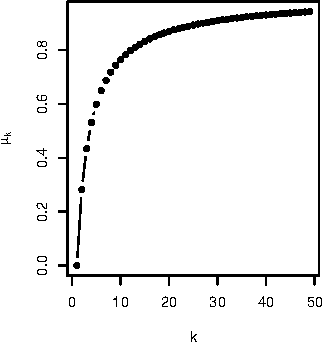
\includegraphics[]{images/nesterov-weights.pdf}
        \caption{%
          Optimal momentum for Nesterov acceleration (for GD).
        }
      \end{figure}

    \end{column}
  \end{columns}
\end{frame}

\begin{frame}[c]
  \frametitle{Convergence}
  \begin{columns}
    \begin{column}{0.45\textwidth}
      Convergence rate with Nesterov acceleration goes from $O(1/k)$ to $O(1/k^2)$

      \medskip\pause

      This is \alert{optimal} for a first-order method.

      \medskip\pause

      Convergence improves further for quadratic and strongly convex!

    \end{column}
    \begin{column}{0.45\textwidth}
      \begin{figure}[htpb]
        \centering
        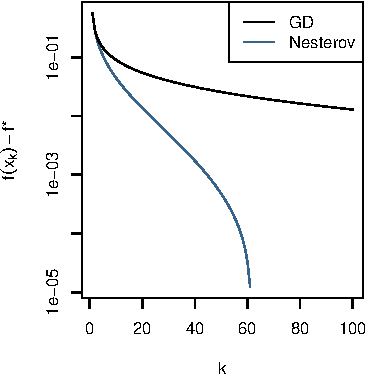
\includegraphics[]{images/momentum-convergence.pdf}
        \caption{%
          Suboptimality plot for a
          logistic regression problem with $n = 1\,000$, $p = 100$.
        }
      \end{figure}
    \end{column}
  \end{columns}

\end{frame}

\begin{frame}[fragile]
  \frametitle{Exercise: Rosenbrock's Banana}

  \begin{block}{Steps}
    \begin{enumerate}
      \item Minimize \[
              f(x_1, x_2) = (a - x_1)^2 + b(x_2 - x_1^2)^2
            \]
            with $a = 1$ and $b = 100$
            using GD with Polyak momentum. Optimum is $(a, a^2)$.
      \item Implement gradient descent.
      \item Add Polyak momentum.
    \end{enumerate}
  \end{block}

  \pause

  \begin{columns}
    \begin{column}{0.45\textwidth}
      \begin{algorithm}[H]
        \KwData{$\gamma >0$, $\mu \in [0,1)$}
        \For{$k \gets 1, 2, \dots$}{
          $x_k \gets x_{k-1} - \gamma  \nabla f(x_{k-1}) + \mu (x_{k-2} - x_{k-2}) $\;
        }
        \caption{GD with Polyak Momentum}
      \end{algorithm}
    \end{column}

    \pause

    \begin{column}{0.45\textwidth}
      \begin{block}{Plot Contours}
        \begin{lstlisting}[language=R]
          x1 <- seq(-2, 2, length.out = 100)
          x2 <- seq(-1, 3, length.out = 100)
          z <- outer(x1, x2, f)
          contour(x1, x2, z, nlevels = 20)
        \end{lstlisting}
      \end{block}
    \end{column}
  \end{columns}

  \pause\bigskip

\end{frame}

\begin{frame}[c]
  \frametitle{What About SGD?}
  So far, we have mostly talked about standard GD, but we can use momentum (Polyak or Nesterov)
  for SGD as well.

  \bigskip

  For standard GD, Nesterov is the dominating method for
  achieving acceleration; for SGD, Polyak momentum is actually
  quite common.

  \bigskip

  In term of convergence, all bets are now off.

  \bigskip

  No optimal rates anymore, just heuristics.
\end{frame}

\begin{frame}[c]
  \frametitle{Adaptive Gradients}

  \begin{block}{General Idea}
    Some directions may be important, but feature information is \alert{sparse}.
  \end{block}

  \pause\bigskip

  \begin{columns}
    \begin{column}{0.45\textwidth}
      \begin{block}{AdaGrad}
        Store matrix of gradient history,
        \[
          G_k = \sum_{i = 1}^k \nabla f(x_k) \nabla f(x_k)^\intercal,
        \]
        and update by multiplying gradient with $G_k^{-1/2}$.
      \end{block}
    \end{column}
    \begin{column}{0.45\textwidth}
      \begin{algorithm}[H]
        \KwData{$\gamma >0$}
        \For{$k \gets 1, 2, \dots$}{
        $G_k \gets G_{k-1} + \nabla f(x_{k-1}) \nabla f(x_{k-1})^\intercal$\;
        $x_k \gets x_{k-1} - \gamma G_k^{-1/2} \nabla f(x_{k-1})$\;
        }
        \caption{AdaGrad}
      \end{algorithm}
    \end{column}
  \end{columns}

  \pause\bigskip

  \begin{block}{Effects}
    Larger learning rates for sparse features

    \medskip

    Step-sizes adapt to curvature.
  \end{block}


\end{frame}

\begin{frame}[c]
  \frametitle{AdaGrad In Practice}

  \begin{block}{Simplified Version}
    Computing \(\nabla f \nabla f^\intercal\) is \(O(p^2)\); expensive!

    \medskip

    Replace \(G^{-1/2}_k\) with \(\diag(G_k)^{-1/2}\)
  \end{block}

  \pause\bigskip

  \begin{block}{Avoid Singularities}
    Add a small \(\epsilon\) to diagonal.
  \end{block}

  \pause\bigskip

  \begin{algorithm}[H]
    \KwData{$\gamma >0$, $\epsilon > 0$}
    \For{$k \gets 1, 2, \dots$}{
      $G_k \gets G_{k-1} + \diag\big(\nabla f(x_{k-1})^2\big)$\;
      $x_k \gets x_{k-1} - \gamma \diag\big(\epsilon I_p + G_k\big)^{-1/2} \nabla f(x_{k-1})$\;
    }
    \caption{Simplified AdaGrad}
  \end{algorithm}

\end{frame}

\begin{frame}[c]
  \frametitle{RMSProp}

  Acronym for \textbf{R}oot \textbf{M}ean \textbf{S}quare \textbf{Prop}agation.

  \begin{block}{Idea}
    Divide learning rate by running average of magnitude of recent gradients:
    \[
      v(x,k) = \xi v(x, k -1) + (1 - \xi)\nabla f(x_k)^2
    \]
    where \(\xi\) is the \alert{forgetting factor}.
  \end{block}

  \medskip

  Similar to AdaGrad, but uses \alert{forgetting} to gradually decrease influence of old data.

  \bigskip

  \begin{algorithm}[H]
    \KwData{$\gamma >0$, $\xi > 0$}
    \For{$k \gets 1, 2, \dots$, $\xi \in [0, 1)$}{
    $v_k = \xi v_{k-1} + (1 - \xi) \nabla f(x_{k-1})$\;
    $x_k \gets x_{k-1} - \frac{\gamma}{\sqrt{v_k}} \odot \nabla f(x_{k-1})$\;
    }
    \caption{RMSProp}
  \end{algorithm}

\end{frame}

\begin{frame}[c]
  \frametitle{ADAM}

  Acronym for \textbf{Ada}ptive \textbf{m}oment estimation

  \medskip

  Basically RMSProp + \emph{momentum} (for both gradients and second moments theorof)

  \medskip

  Popular and still in much use today.

\end{frame}

\begin{frame}[c]
  \frametitle{Implementation Aspects of SGD}

  \begin{block}{Loops}
    Any language (e.g. R) that imposes overhead for loops, will have a difficult time with SGDS
  \end{block}

  \pause

  \begin{block}{Storage Order}
    In a regression setting, when indexing a single obervation at a time, slicing rows is not efficient
    $n$ is large.

    \medskip

    We can either transpose first or use a row-major storage order (not possible in R).
  \end{block}
\end{frame}

\begin{frame}[c]
  \frametitle{Example: Nonlinear Least Squares}

  \begin{columns}
    \begin{column}{0.42\textwidth}
      Let's assume we're trying to solve a least-squares type of problem:
      $$f(\theta) = \frac{1}{2n} \sum_{i=1}^n  \left(y_i - g(\theta; x_i, y_i)\right)^2$$
      with $\theta = (\alpha, \beta)$ and
      $$g(\theta; x, y) = \alpha \cos(\beta x).$$

      \bigskip\pause

      Then
      \[
        \nabla_{\theta} f(\theta) =
        \begin{bmatrix}
          \cos(\beta x) \\ - \alpha x \sin(\beta x)
        \end{bmatrix}.
      \]
    \end{column}
    \begin{column}{0.5\textwidth}
      \begin{figure}[htpb]
        \centering
        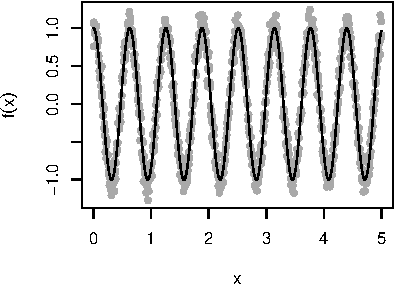
\includegraphics[]{images/nonlinear-data.pdf}
        \caption{%
          Simulation from problem
        }
      \end{figure}
    \end{column}
  \end{columns}
\end{frame}

\begin{frame}[c]
  \begin{columns}
    \begin{column}{0.4\textwidth}
      \begin{figure}[htpb]
        \centering
        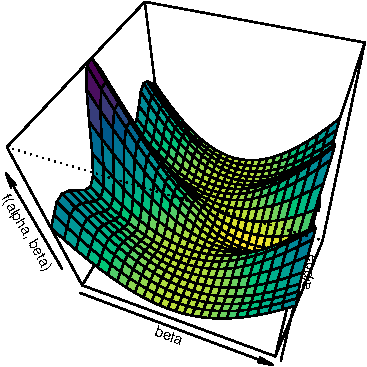
\includegraphics[]{images/nonlinear-persp.pdf}
        \caption{%
          Perspective plot of function
        }
      \end{figure}
    \end{column}
    \pause
    \begin{column}{0.5\textwidth}
      \begin{figure}[htpb]
        \centering
        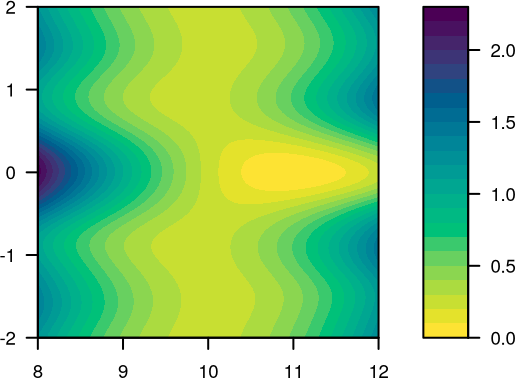
\includegraphics[]{images/nonlinear-contour.png}
        \caption{%
          Contour plot of \(f\)
        }
      \end{figure}
    \end{column}
  \end{columns}
\end{frame}

\begin{frame}[c]
  \begin{figure}[htpb]
    \centering
    \multiinclude[<+>][format=pdf]{images/nonlinear-convergence}
    \caption{%

    }
  \end{figure}
\end{frame}

\begin{frame}[c]
  \begin{figure}[htpb]
    \centering
    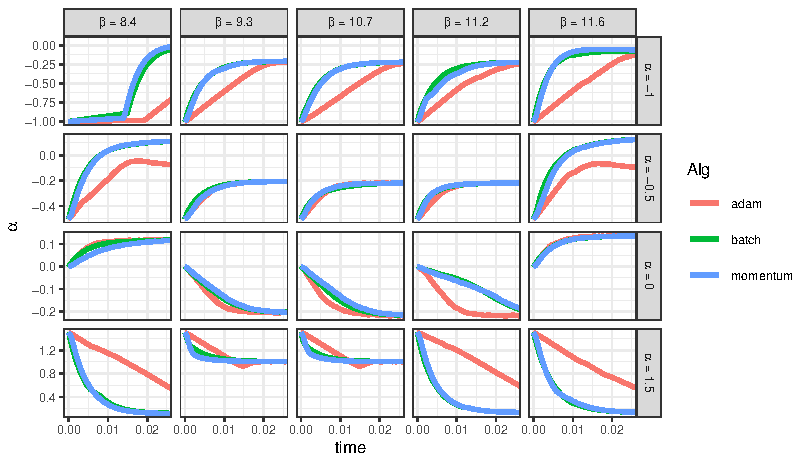
\includegraphics[]{images/nonlinear-alpha.pdf}
    \caption{%
      Updates of \(\alpha\) parameter over time for the different algorithms over
      different starting values.
    }
  \end{figure}

\end{frame}

\begin{frame}[c]
  \begin{figure}[htpb]
    \centering
    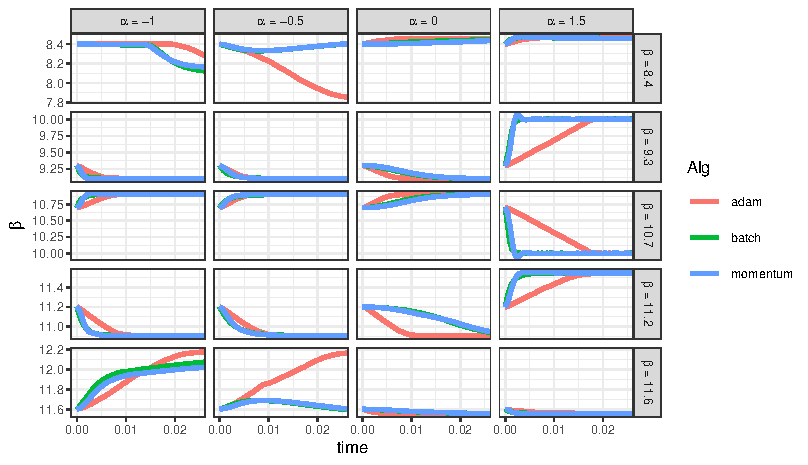
\includegraphics[]{images/nonlinear-beta.pdf}
    \caption{%
      Updates of \(\beta\) parameter over time for the different algorithms over
      different starting values.
    }
  \end{figure}
\end{frame}

\begin{frame}[c]
  \frametitle{Rcpp}

  Very attractive for stochastic methods due to all the loop constructs and slicing.

  \medskip

  However, Rcpp lacks linear algebra functions.

  \begin{block}{Approaches}
    \begin{itemize}
      \item Still use only Rcpp (but then you need to write your own linear algebra functions\footnote{Not recommended!}
      \item Use RcppEigen or RcppArmadillo.
    \end{itemize}
  \end{block}
\end{frame}

\begin{frame}[c]
  \frametitle{Exercise: Rosenbrock Revisited}

  \begin{block}{Steps}
    \begin{enumerate}
      \item Convert your gradient descent algorithm to C++ through Rcpp.
      \item Modify it to be a stochastic gradient descent algorithm instead.
    \end{enumerate}
  \end{block}

  \pause\bigskip

  \begin{block}{Hints}
    \begin{itemize}
      \item Use the Rcpp function \texttt{Rcpp::sugar()} to sample indices.
      \item Don't bother with a stopping criterion to begin with; just set a maximum number of
            iterations.
      \item You can return a list by calling \texttt{Rcpp::List::create(Rcpp::named("name") = x)}.
      \item Use a pure Rcpp implementation.
    \end{itemize}
  \end{block}

\end{frame}

\begin{frame}[c]
  \frametitle{Summary}

  We introduced several new concepts:
  \begin{itemize}
    \item Polyak momentum,
    \item Nesterov acceleration (momentum), and
    \item adapative gradients (AdaGrad),
  \end{itemize}

  \bigskip

  We practically implemented versions of gradient descent and stochastic gradient
  descent with momentum.

  \pause\bigskip

  \begin{block}{Additional Resources}
    \begin{itemize}
      \item \textcite{gohWhyMomentumReally2017} is a article on momentum
            in gradient descent with lots of interactive visualizations.
    \end{itemize}
  \end{block}
\end{frame}


\begin{frame}[c]
  \frametitle{Next Time}

  \begin{block}{Reproducibility}
    How to make your code reproducible

    \medskip

    We build an R package.
  \end{block}

  \pause

  \begin{block}{Summary}
    We summarize the course.
  \end{block}

  \pause

  \begin{block}{Exam Advice}
    We talk about the upcoming oral examinations.
  \end{block}

\end{frame}

\begin{frame}[standout]
  Thank you!
\end{frame}

\appendix

\begin{frame}[allowframebreaks]{References}
  \printbibliography[heading=none]
\end{frame}


\end{document}

